\begin{figure}[H]
\centering
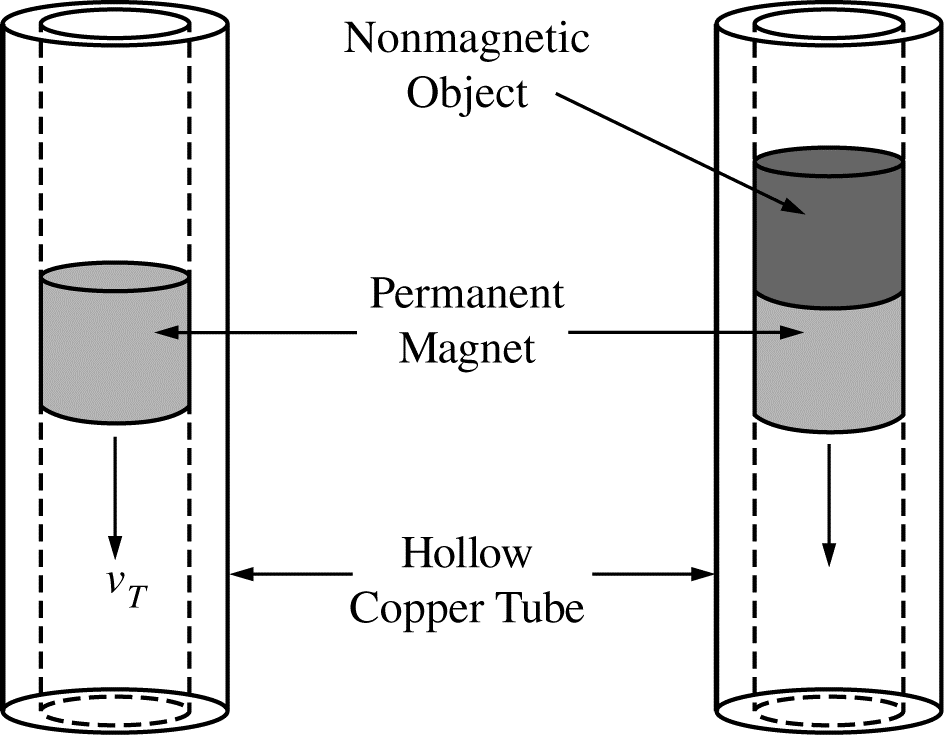
\includegraphics[scale=0.25]{images/img-010-032.png}
\end{figure}

% Multiple Choice Question 20
\begin{questions}\setcounter{question}{19}\question
A permanent magnet of mass $M$ is dropped down the interior of a hollow cylindrical tube made of copper, as shown at left in the figure above. Friction between the inside of the tube and the magnet is negligible. As the magnet moves downward, an upward magnetic force $F_{B}$ is induced, and the magnet's velocity quickly reaches a constant terminal value $v_{T}$. A nonmagnetic object of mass $M$ is attached to the permanent magnet and the drop is repeated, as shown at right in the figure above. When terminal velocity is reached, how do the new values of $F_{B}$ and $v_{T}$ compare with their values without the object?

\begin{choices}
\choice $F_{B}$ and $v_{T}$ are the same.
\choice $F_{B}$ is larger and $v_{T}$ is smaller.
\choice $F_{B}$ is smaller and $v_{T}$ is larger.
\choice $F_{B}$ and $v_{T}$ are both larger.
\choice $F_{B}$ and $v_{T}$ are both smaller.
\end{choices}\end{questions}

